% \begin{savequote}[8cm]
% \textlatin{Neque porro quisquam est qui dolorem ipsum quia dolor sit amet, consectetur, adipisci velit...}

% There is no one who loves pain itself, who seeks after it and wants to have it, simply because it is pain...
%   \qauthor{--- Cicero's \textit{de Finibus Bonorum et Malorum}}
% \end{savequote}

\chapter{\label{ch:1-intro}Introduction} 

\minitoc
% \newpage



Proteins are the molecular building blocks of all living systems. The emergence of life from these fundamental components depends on how proteins are organised in both space and time, and across a magnitude of scales. Understanding the forces governing this organisation not only elucidates how matter comes alive, but knowing how and why these processes go wrong can help us to design effective therapeutics for disease or even hijack and engineer these processes to harness the power of proteins.

In this thesis I explore three different mechanisms for protein organisation. I will develop mathematical models that capture the main features of physical interactions between proteins and study the structure and consequences of these equations, comparing with experimental studies where relevant. Each mechanism has broadly been studied before but I will detail how previous studies have failed to capture key features of the interaction that can lead to a fundamentally different route for protein organisation.

\section{What is a protein?}

Biochemically, proteins are a class of molecules that are long unbranched chains of monomer units, called amino acids. \cite{jones2002soft} Each amino acid has the same basic structure that polymerises to form a protein backbone held together by peptide bonds, a type of covalent bond. The distinct amino acids have distinct side chains that are attached to the polymerising unit and it is this side chain that defines the different amino acids. This sequence of amino acids, including their side chains, defines the protein and is referred to as the primary protein structure. \cite{alberts_molecular_2008} The sequence of amino acids in the primary structure is stored in the genetic information of each organism and is passed down through generations. Various cellular machinery, read this genetic information and manufacture polypeptide chains. An array of non-covalent bonds, such as hydrogen bonds, electrostatic attractions and van der Waals, then determine how the protein is \textit{folded}, that is, the resulting configuration of the chain in 3D space or the protein's \textit{ternary structure}. This ternary structure defines the shape of the protein, and specifies the location of each atom, although thermal fluctuations induce slight perturbations and prevent proteins from being fixed in this exact configuration. The protein's ternary structure is also crucial in determining the proteins function, for example proteins that catalyse biological reactions, enzymes, do so by binding to a molecule to form a complex. The lock and key model of this binding requires that the enzyme and molecule have exactly complimentary shapes. \cite{berg_biochemistry_2002}

\subsection{The Hierarchy of Protein Interactions}

\begin{figure}
    \centering
    % 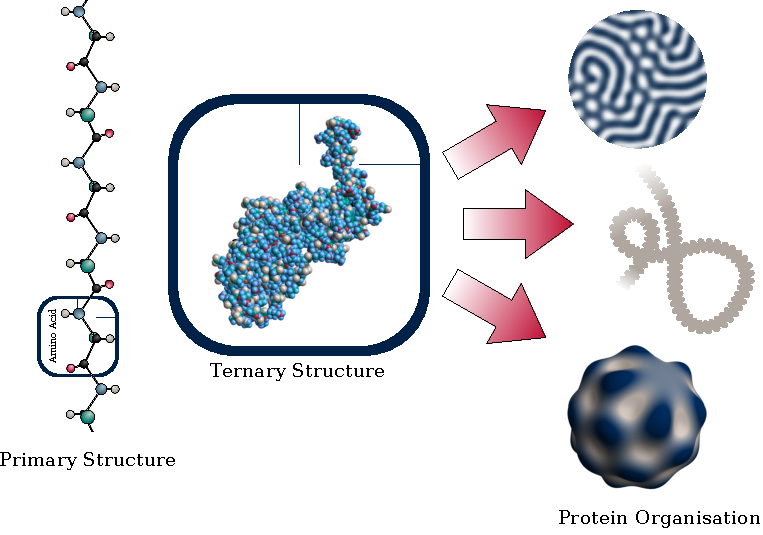
\includegraphics[width=0.8\textwidth]{figures/1-intro-figs/proteinLevels.pdf}
    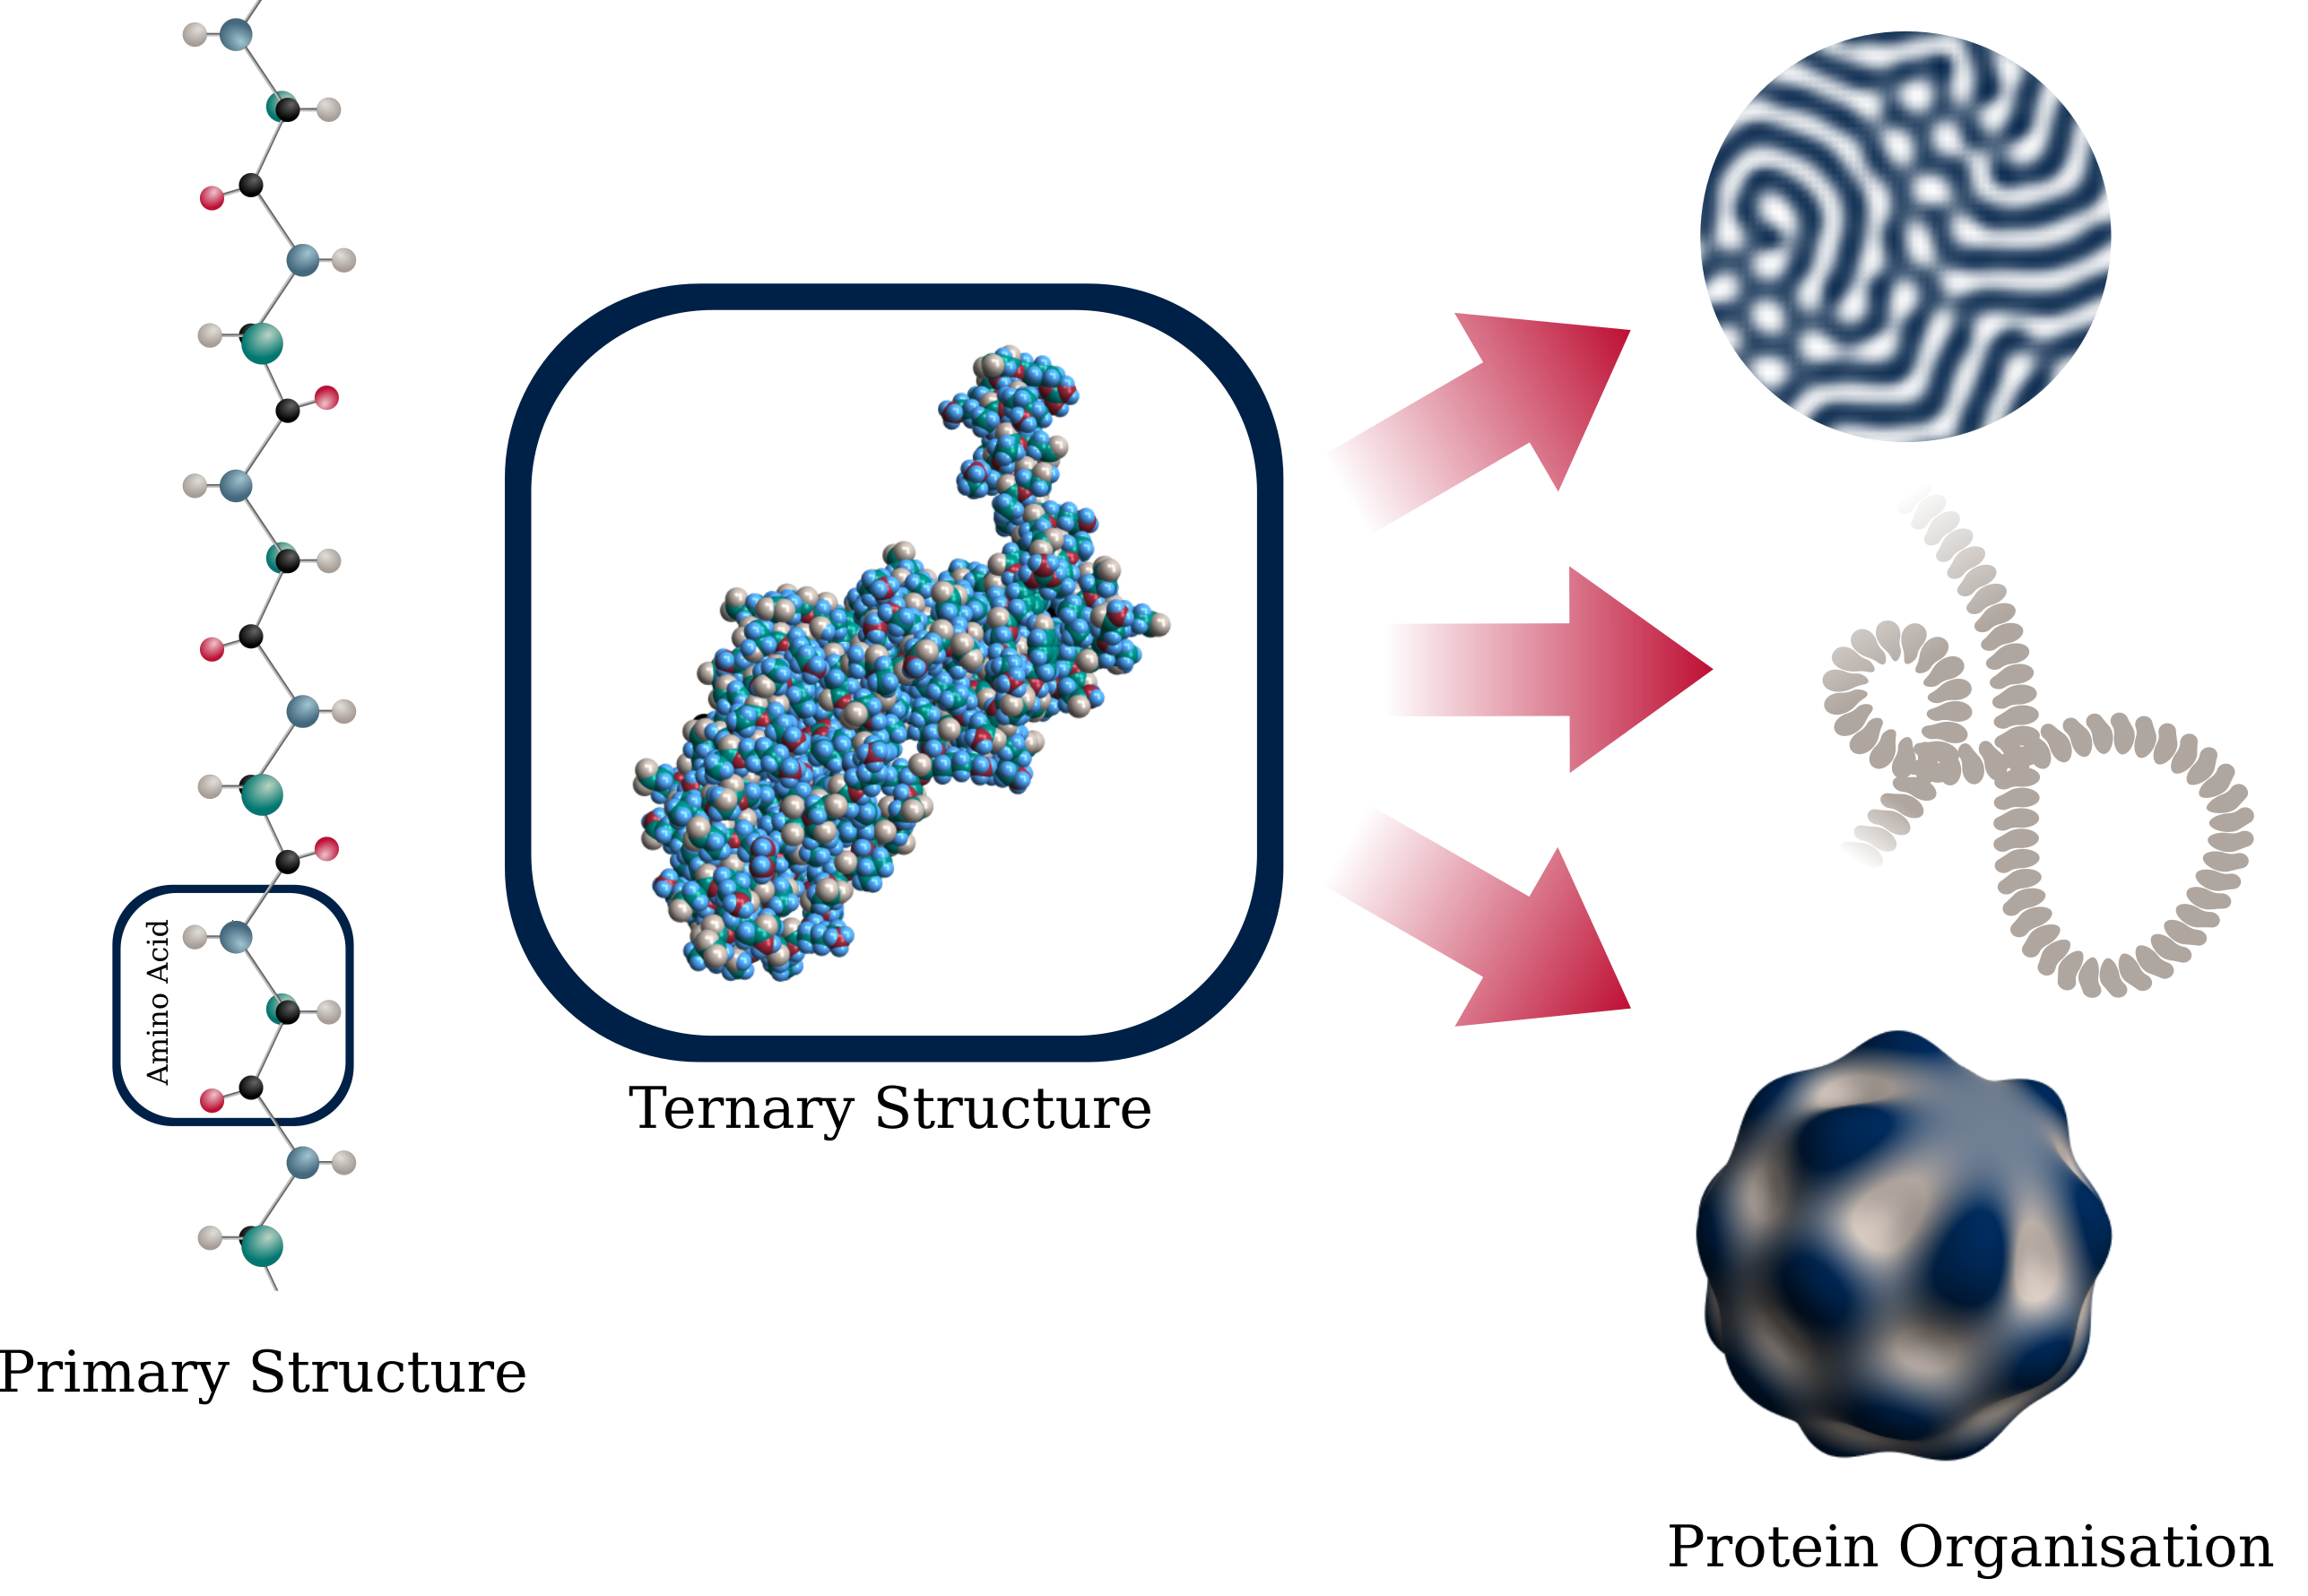
\includegraphics[width=1\textwidth]{figures/1-intro-figs/proteinLevels.png}
    \caption{The hierarchy of protein structure. Amino acids make proteins that then interact to form structures and patterns. The graphics show examples of protein organisation inspired by (top to bottom) reaction diffusion systems \cite{turing_chemical_1952}, fibrils \todo{ref} and curvature induced membrane patterning \cite{agudo-canalejo_pattern_2017}. The structure of the protein shown is generated from coordinates in the protein database, structure 1EZB, \cite{garrett_solution_1997}}
    \label{fig:1-proteinLevels}
\end{figure}

During my DPhil the development and release of AlphaFold changed the conversation around protein structure. AlphaFold is a neural network desigened to solve the problem of protein folding: learning the map from amino acid sequence (primary structure) to an atomistic description of the 3D shape (ternary structure). In 2021, AlphaFold became the first computational method to achieve accuracy on par with experimental structure determination. \cite{jumper_highly_2021} Since then, it has become an invaluable tool in the arsenal of scientists trying to understand a variety of biological processes. Structure prediction can help to understand why, for example, a genetic modification might stop a molecule binding to a protein, elucidating unknown binding mechanisms, and engineering mutations to enhance binding affinity and catalytic rates. This model also represented a paradigm shift from mechanistic physics informed modelling to solve the folding problem to a deep learning approach. This was possible due to the extensive database of experimentally determined structures in the Protein Data Bank and the abundance of sequencing data from advanced sequencing technologies.

In this thesis, I have explored an alternative approach to protein engineering and I have explored interactions at a different scale. Rather than considering changing the individual protein structure, I have explored mechanisms by which proteins can conspire to form structures that affect function. This collective organisation often relates to protein structure, however my research demonstrates that the protein environment also plays a crucial role in tuning emergent phenomena. Varying monomer concentration in systems of aggregating proteins, adding solvent to a dense active mixture, or increasing the tension in a membrane filled with proteins are all examples of the rich parameter space that can be explored when we begin to understand larger scale protein dynamics.

% \subsection{Abstracting and Modelling Proteins}

% The space of amino acid chains and therefore of potential proteins is vast. There are 20 distinct amino acids that form chains of typically 50---2000 amino acid redisudues long \cite{berg_biochemistry_2002} and so for a relatively short chain of 100 residues, there are $20^{100} \approx 10^{130}$ possible different chain sequences. A lot of these sequences wouldn't form a stable 3D structure, but this quick calculation demonstrates the massive protein design space that evolution has been able to explore.

% As such, proteins are a fantastic model system for mathematicians and physicists to study. At some spatial scales, they are small enough to abstract as simple particles susceptible to coarse grainging and contimuum limits. , but have sufficient complexity that they can interact in a multitude of ways, either with other proteins, other molecules, of with the broader environment. This is exactly the 

% Mutliscale system

% In some conditions the systems is made up of 

% Models of colloidal systems apply to proteins.

% and near endless fun for mathematicians and physicists

\section{Proteins in Health and Disease}

Proteins are the work horses of cellular and subcellular machinery. If anything happens on the subcelluar scale, there is normally a protein making to happen. Enzymes are proteins that catalyse reactions, making processes feasible on relevant molecular timescales. \cite{alberts_molecular_2008} Kinesin and other motor proteins drag cargo and provide essential active transport functionality, \cite{hirokawa_molecular_2010} however proteins such as ion channels can span barriers within the cell and allow passive transport to occur. \cite{berg_biochemistry_2002} This arsenal of transport processes determines how the distribution of biomolecules is kept from equilibrium, or how efficiently a system can relax to some steady state, helping to control cell signalling and the flow of information.

Another function of proteins is as building blocks for subcellular structures such as microtubules or viral capsids. \cite{keskin_principles_2008} In recent years, liquid-liquid phase separation has also emerged as a key feature of intracellular organisation \cite{shin, banani_biomolecular_2017}. These are liquid droplets that have a different composition to the surrounding environment, typically with an enriched protein concentration. The droplets, or condensates, can act as reaction crucibles, can promote signalling or sequester molecules in the cell and prevent off target effects. \cite{shin_liquid_2017} The formation and maturation of liquid condensates are entirely governed by protein interactions.

The importance of proteins in so many biological processes means that they can have devastating effects when the fail to function correctly. For example, cystic fibrosis is a disease caused by the misfolding of a transmembrane protein and subsequent its inability to function. \cite{luheshi_protein_2008} In addition to this lack of function mechanism, the gain of toxic function can also cause disease. \cite{dobson_protein_2003} A whole class of diseases stem from proteins interacting and forming toxic aggregates. \cite{chiti_protein_2006, chiti_protein_2017} Understanding how essential, functional protein-protein interactions may go awry, or how toxic interactions emerge, is essential to understanding and preventing many human diseases.

\section{Engineering Proteins}

Proteins serve as the foundation for many engineered biomaterials, with keratin being a prominent example. Keratin is a naturally occurring fibrous protein found in hair, nails, feathers, and horns.\cite{sharma_keratin_2019} Keratin-based biomaterials have a wide range of biomedical applications, including wound dressings, tissue engineering scaffolds, and drug delivery systems.\cite{feroz_keratin_2020} The protein forms long, cross-linked filaments that can be either hard or soft, depending on the sulfur content of the material. Sulfur, or in some cases other proteins, create cross-links between keratin filaments, with these interactions determining the strength and structure of the resulting material creating, fibers, films, sponges, gels, or scaffolds. The utility of keratin-based biomaterials lies in their ability to self-assemble into 3D structures, a process entirely governed by protein interactions.\cite{feroz_keratin_2020}

Multi-component engineered systems also include proteins as key component. Synthetic membranes that act as controllable barriers, rely on  on protein interactions with the membranes for effective embedding and manufacture. \cite{garni_bioporesmembrane_2017} Such membranes can support the development of nanoreactors, artificial organelles or chemically active surfaces. Proteins can also interact with membranes to transport cargo allowing for spatial organisation with applications to creating synthetic cells and mimicking lifelike function \cite{ramm_diffusiophoretic_2021}. The whole field of synthetic biology is built around controlling and programming cell-like behaviour and proteins are a necessary tool in this pursuit. \cite{cameron_brief_2014}

% Outside of direct applications, proteins are key components in assays and platform technologies. For example, the green fluorescent protein (GFP) from a species of jellyfish that emits a \todo{color etc}. \cite{tsien_green_1998} GFP has been used to detect gene expression or phosphorylation, or to detect protein-protein interactions. PCR? synbio etc.

\section{Thesis Scope and Structure}

Each chapter in this thesis explores a different physical mechanism to drive protein organisation. I will introduce the background necessary to understand each mechanism and highlight specific aspects of these protein-protein interactions that have been previously understudied. Using a range of techniques, I will build mathematical models that incorporate important featurs of the interactions and study the effects on the resulting protein organisation, ultimately exploring how this can affect function or pathology. Below I provide a very brief summary of each system studied:
\begin{enumerate}
    \item \textbf{Catalysis Induced Phase Separation} Liquid-liquid phase separation can form droplets in mixtures of proteins and other components. The formation of these regions can be driven by equilibrium interactions between the components, but in this chapter I demonstrate that modelling chemically active components can give rise to fundamentally new phenomena. An enzymatic component can drive liquid-liquid phase separation without the interactions and this can subsequently affect overall reaction rates in the system.
    \item \textbf{Anisotropic Membrane Mediated Interactions} Proteins that bind to and bend biological membranes can generate elastic forces that act on other proteins in the membrane. These forces can generate structures and remodel the membrane. However, many of the proteins that bind in this way break radial symmetry and this changes their interactions, introducing an equilibrium separation and forming lattices of inclusions that can be controlled via the protein curvature or membrane stiffness.
    \item \textbf{Bounded clearance in Neurodegenerative Disease} A plethora of neurodegenrative diseases are associated with aggregated proteins that are produced and removed in the brain. However, existing models ignore physical constraints that limit and bound the rates at which these aggregated proteins can be removed. Including this key limit when modelling the aggregation kinetics can present a fundamentally new mechanism for the onset of disease which is consistent with recent experiments and can help design rational therapeutics.
\end{enumerate}